\documentclass[a4paper, 12pt]{article}		% general format

%%%% Charset
\usepackage{cmap}							% make PDF files searchable and copyable
\usepackage[utf8]{inputenc}					% accept different input encodings
\usepackage[T2A]{fontenc}					% russian font
\usepackage[russian]{babel}					% multilingual support (T2A)

%%%% Graphics
\usepackage[dvipsnames]{xcolor}			% driver-independent color extensions
\usepackage{graphicx}						% enhanced support for graphics
\usepackage{wrapfig}						% produces figures which text can flow around

%%%% Math
\usepackage{amsmath}						% American Mathematical Society (AMS) math facilities
\usepackage{amsfonts}						% fonts from the AMS
\usepackage{amssymb}						% additional math symbols

%%%% Typograpy (don't forget about cm-super)
\usepackage{microtype}						% subliminal refinements towards typographical perfection
\linespread{1.3}							% line spacing
\usepackage[left=2.5cm, right=1.5cm, top=2.5cm, bottom=2.5cm]{geometry}
\setlength{\parindent}{0pt}					% we don't want any paragraph indentation
\usepackage{parskip}
%\renewcommand{\chaptername}{}

%%%% Other
\usepackage{url}							% verbatim with URL-sensitive line breaks
%\DeclareUnicodeCharacter{00A0}{~}

%------------------------------------------------------------------------------
\usepackage{listings}						% typeset source code listings

% Цвета для кода
\definecolor{string}{HTML}{101AF9}			% цвет строк в коде
\definecolor{comment}{HTML}{3F7F5F}		% цвет комментариев в коде
\definecolor{keyword}{HTML}{5F1441}		% цвет ключевых слов в коде
\definecolor{morecomment}{HTML}{8000FF}	% цвет include и других элементов в коде
\definecolor{captiontext}{HTML}{FFFFFF}	% цвет текста заголовка в коде
\definecolor{captionbk}{HTML}{999999}		% цвет фона заголовка в коде
\definecolor{bk}{HTML}{FFFFFF}				% цвет фона в коде
\definecolor{frame}{HTML}{999999}			% цвет рамки в коде

% Настройки отображения кода
\lstset{
	language=C++,							% Язык кода по умолчанию
	morekeywords={*,...},					% если хотите добавить ключевые слова, то добавляйте
	% Цвета
	keywordstyle=\color{keyword}\ttfamily\bfseries,
	stringstyle=\color{string}\ttfamily,
	commentstyle=\color{comment}\ttfamily\itshape,
	morecomment=[l][\color{morecomment}]{\#},
	% Настройки отображения
	breaklines=true,						% Перенос длинных строк
	basicstyle=\ttfamily\footnotesize,		% Шрифт для отображения кода
	backgroundcolor=\color{bk},				% Цвет фона кода
	%frame=lrb,xleftmargin=\fboxsep,xrightmargin=-\fboxsep, % Рамка, подогнанная к заголовку
	frame=tblr								% draw a frame at all sides of the code block
	rulecolor=\color{frame},				% Цвет рамки
	tabsize=2,								% tab space width
	showstringspaces=false,					% don't mark spaces in strings
	% Настройка отображения номеров строк. Если не нужно, то удалите весь блок
	numbers=left,							% Слева отображаются номера строк
	stepnumber=1,							% Каждую строку нумеровать
	numbersep=5pt,							% Отступ от кода
	numberstyle=\small\color{black},		% Стиль написания номеров строк
	% Для отображения русского языка
	extendedchars=true,
	literate={Ö}{{\"O}}1
	 	{Ä}{{\"A}}1
	 	{Ü}{{\"U}}1
		{ß}{{\ss}}1
		{ü}{{\"u}}1
		{ä}{{\"a}}1
		{ö}{{\"o}}1
		{~}{{\textasciitilde}}1
		{а}{{\selectfont\char224}}1
		{б}{{\selectfont\char225}}1
		{в}{{\selectfont\char226}}1
		{г}{{\selectfont\char227}}1
		{д}{{\selectfont\char228}}1
		{е}{{\selectfont\char229}}1
		{ё}{{\"e}}1
		{ж}{{\selectfont\char230}}1
		{з}{{\selectfont\char231}}1
		{и}{{\selectfont\char232}}1
		{й}{{\selectfont\char233}}1
		{к}{{\selectfont\char234}}1
		{л}{{\selectfont\char235}}1
		{м}{{\selectfont\char236}}1
		{н}{{\selectfont\char237}}1
		{о}{{\selectfont\char238}}1
		{п}{{\selectfont\char239}}1
		{р}{{\selectfont\char240}}1
		{с}{{\selectfont\char241}}1
		{т}{{\selectfont\char242}}1
		{у}{{\selectfont\char243}}1
		{ф}{{\selectfont\char244}}1
		{х}{{\selectfont\char245}}1
		{ц}{{\selectfont\char246}}1
		{ч}{{\selectfont\char247}}1
		{ш}{{\selectfont\char248}}1
		{щ}{{\selectfont\char249}}1
		{ъ}{{\selectfont\char250}}1
		{ы}{{\selectfont\char251}}1
		{ь}{{\selectfont\char252}}1
		{э}{{\selectfont\char253}}1
		{ю}{{\selectfont\char254}}1
		{я}{{\selectfont\char255}}1
		{А}{{\selectfont\char192}}1
		{Б}{{\selectfont\char193}}1
		{В}{{\selectfont\char194}}1
		{Г}{{\selectfont\char195}}1
		{Д}{{\selectfont\char196}}1
		{Е}{{\selectfont\char197}}1
		{Ё}{{\"E}}1
		{Ж}{{\selectfont\char198}}1
		{З}{{\selectfont\char199}}1
		{И}{{\selectfont\char200}}1
		{Й}{{\selectfont\char201}}1
		{К}{{\selectfont\char202}}1
		{Л}{{\selectfont\char203}}1
		{М}{{\selectfont\char204}}1
		{Н}{{\selectfont\char205}}1
		{О}{{\selectfont\char206}}1
		{П}{{\selectfont\char207}}1
		{Р}{{\selectfont\char208}}1
		{С}{{\selectfont\char209}}1
		{Т}{{\selectfont\char210}}1
		{У}{{\selectfont\char211}}1
		{Ф}{{\selectfont\char212}}1
		{Х}{{\selectfont\char213}}1
		{Ц}{{\selectfont\char214}}1
		{Ч}{{\selectfont\char215}}1
		{Ш}{{\selectfont\char216}}1
		{Щ}{{\selectfont\char217}}1
		{Ъ}{{\selectfont\char218}}1
		{Ы}{{\selectfont\char219}}1
		{Ь}{{\selectfont\char220}}1
		{Э}{{\selectfont\char221}}1
		{Ю}{{\selectfont\char222}}1
		{Я}{{\selectfont\char223}}1
		{і}{{\selectfont\char105}}1
		{ї}{{\selectfont\char168}}1
		{є}{{\selectfont\char185}}1
		{ґ}{{\selectfont\char160}}1
		{І}{{\selectfont\char73}}1
		{Ї}{{\selectfont\char136}}1
		{Є}{{\selectfont\char153}}1
		{Ґ}{{\selectfont\char128}}1
}

% Для настройки заголовка кода
\usepackage{caption}
\DeclareCaptionFont{white}{\color{сaptiontext}}
\DeclareCaptionFormat{listing}{\parbox{\linewidth}{\colorbox{сaptionbk}{\parbox{\linewidth}{#1#2#3}}\vskip-4pt}}
%\captionsetup[lstlisting]{format=listing,labelfont=white,textfont=white}
\renewcommand{\lstlistingname}{Листинг} % Переименование Listings в нужное именование структуры

%------------------------------------------------------------------------------
\begin{document}

\begin{titlepage}
\thispagestyle{empty}

\begin{center}
Санкт-Петербургский государственный политехнический университет \\
Институт Информационных Технологий и Управления \\*
Кафедра компьютерных систем и программных технологий \\*
\hrulefill
\end{center}

\vspace{18em}

\begin{center}
\Large Отчёт по практической работе\\ по предмету «Системное программное обеспечение» \\
\end{center}

\vspace{1em}

% \linebreak
\begin{center}
\textsc{\textbf{Утилита top}}
\end{center}

\vspace{16em}

\begin{flushleft}
Работу выполнил студент гр. 53501/3\hrulefill Мартынов С. А. \\
\vspace{1.5em}
Работу принял преподаватель \hrulefill Душутина Е. В. \\
\end{flushleft}

\vspace{\fill}

\begin{center}
Санкт-Петербург \\
2015
\end{center}

\end{titlepage}
%------------------------------------------------
\setcounter{page}{2}
\tableofcontents
%------------------------------------------------
\newpage
\section*{Постановка задачи}
\addcontentsline{toc}{section}{Постановка задачи}

В рамках данной работы необходимо ознакомиться с работой утилиты top. Рассмотреть и описать механизмы сбора информации, используемые системные вызовы и общий порядок функционирования утилиты.
\vspace{3em}

В работе необходимо указать источники и версии используемых программных продуктов.


\newpage
%------------------------------------------------
\section*{Введение}
\addcontentsline{toc}{section}{Введение}

Работа выполняется под управлением Ubuntu 14.04.2 LTS. В качестве изучаемой утилиты используется реализация htop (автор Hisham H. Muhammad). Htop написан на языке Си и использует для отображения библиотеку Ncurses. Htop показывает динамический список системных процессов (рисунок 1), список обычно выравнивается по использованию ЦПУ. В отличие от top, htop показывает все процессы в системе. Также показывает время непрерывной работы, использование процессоров и памяти.

\begin{figure}[h!]
\centering
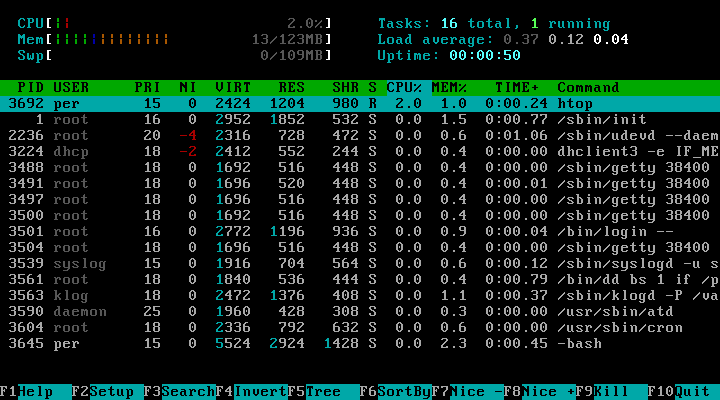
\includegraphics[scale=0.65]{res/Htop}
\caption{Системный монитор htop}
\end{figure}

Рассматривается версия 1.0.3 (от 24 апреля 2014 года). Исходники доступны по лицензии GPL на сайте \url{http://hisham.hm/htop/}. Для простоты изучения, в код системы были внесены не значительные изменения.

Часть кода приведена в листингах, но более подробная версия и отчёт доступны по адресу \\ \url{https://github.com/SemenMartynov/SPbPU_SystemProgramming}.

\newpage
%------------------------------------------------
\section{Виртуальная файловая система procfs}

Файловая система /ргос содержит подробную информацию об активных процессах. Информация о процессе, сохраненная в файловой системе /ргос, изменяется по мере прохождения данным процессом его жизненного цикла.

Каждый элемент в каталоге /ргос - это десятичное число, соответствующее идентификатору какого-нибудь процесса. Каждый каталог в файловой системе /ргос содержит файлы с более подробной информацией о данном процессе. Владелец каждого файла в каталоге /ргос и его подкаталогах устанавливается по номеру идентификатора пользователя данного процесса.

Первоначально procfs была разработана для свободного получения  информации о состоянии процессов, теперь ее функции расширились, и через эту виртуальную файловую систему процессам можно передавать какие-то параметры (см. рис. 2).

\begin{figure}[h!]
\centering
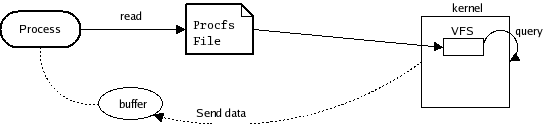
\includegraphics[scale=0.9]{res/ProcessFileSystem}
\caption{Виртуальная файловая система procfs}
\end{figure}

Виртуальной она называется потому, что имеющиеся здесь файлы и каталоги на самом деле не находятся на жестком диске. После загрузки ядра они находятся в оперативной памяти. Для пользователя этот механизм полностью  прозрачен. Многие программы, в  том числе htop, собирают информацию из  файлов  в  /рrос, форматируют их и выводят результат.

В /рrос можно найти  также  информацию об установленном оборудовании,  разметке  жесткого диска, статистику и  многое другое.

При работе с /proc есть важный нюанс: информацию  из  файла можно прочитать, но открыть его в текстовом редакторе не получится, т.к. его содержимое может измениться в любую секунду. Для записи  и  считывания данных в  такой  файл используются утилиты, вроде car и echo.

Файлы в  procfs могут иметь три варианта доступа:
\begin{itemize}
\item только для чтения — предназначены для получения информации об определенном параметре, при попытке в них что-то записать будет выдано предупреждение;
\item только для чтения пользователем root — такой же, как и предыдущий, но получить информацию может только администратор;
\item только для записи  пользователем root — позволяет не только считать данные, но и  изменить параметр.
\end{itemize}

Возможны и  некоторые комбинации  этих трех вариантов.  К тому же в  некоторые файлы можно записать только строго определенное значение.

Утилита htop производит считывание различных параметров процессов. Далее будет рассмотрено как это происходит.


\newpage
%------------------------------------------------
\section{Процессы}

Листинг 1 содержит отрывок файла Process.h, описывающий структуру Process. На самом деле этот отрезок короче, если учесть работу препроцессора, который содержит многие строки (отладочную информацию, данные OpenVZ и виртуального сервера).

\lstinputlisting[firstline=63,lastline=153,language=C++, caption={Клиент именованного каналов}]{../../top/Process.h}

Назначение большинства полей понятно исходя из их названий, и они здесь представлены для дальнейшего перехода к системам, которые заполняют значение этих полей (к примеру, процент занятой памяти или процессорного времени). Процессы объединяются в списки (строка 4), а объект Object (строка 2) отвечает за отображение. Полный граф взаимодействия структура данных представлен на рисунке 3.

\begin{figure}[h!]
\centering
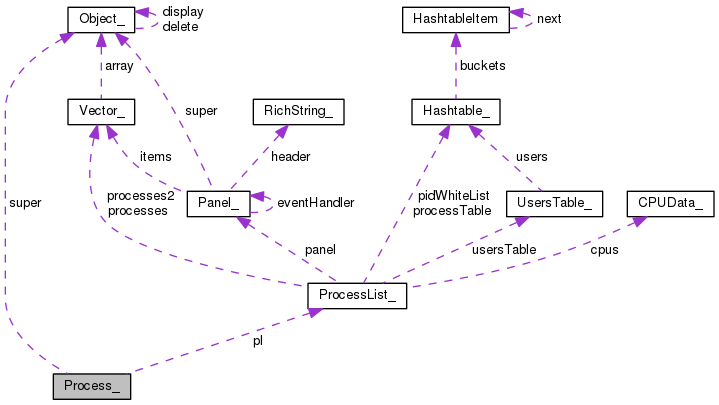
\includegraphics[scale=0.7]{res/process.png}
\caption{Граф взаимодействия для структуры Process}
\end{figure}

На графе видно, что некоторые структуры, такие как CPUData\_ не связаны с конкретным процессом, и это логично, т.к. эта общесистемная информация, но к ней есть доступ через сам список. Структуры, такие как RitcString\_, Vector\_ и Hashtable\_ используются для служебных целей (сортировка списков, парсинг текстовой информации), т.к. программа написана на C (т.е. это реализация структур из C++, реализованная на языке С).

Все процессы помещаются в список, который, помимо самих процессоров, хранит ещё общесистемные показатели, такие как распределение памяти и ресурсов центрального процессора (листинг 2).

Получить показатели используемой памяти можно из файла /proc/meminfo (стр. 5 - макрос подставит правильный путь на место PROCMEMINFOFILE). В этой функции определяется следующие показатели памяти:
\begin{itemize}
\item общий объём памяти (стр 17);
\item объём свободной памяти (стр. 19);
\item объём памяти, разделяемой между процессами (стр. 21);
\item размер буферов (стр. 25);
\item размер кешей (стр.29);
\item общий объём, используемый для хранения страниц памяти на диске (стр. 33);
\item свободное место в свапе (стр. 35);
\item объём используемой памяти, как разность между общим объёмом и свободной памятью (стр. 41);
\item объём используемого места в свапе, как разность между общим объёмом и свободным пространством (стр. 42);
\end{itemize}

Помимо информации о памяти, тут же происходит считывание информации о прерываниях и операциях ввода-вывода из файла /proc/stat (стр. 45 - замена имени файла будет произведена препроцессором). из этого файла для каждого процессора (стр. 49) считываются следующие показатели:
\begin{itemize}
\item время, проведённое процессором в пространстве пользователя (стр. 83);
\item время, на выделение которого повлиял приоритет процесса (стр. 84);
\item время, проведённое процессором в пространстве ядра (стр. 85);
\item время, проведённое процессором в пространстве ядра, включая обработку прерываний (стр. 86);
\item время, проведённое процессором в режиме бездействия (стр. 87);
\item время, проведённое процессором в режиме бездействия, включая время ожидания выполнения операций ввода-вывода (стр. 88);
\item время ожидания выполнения операций ввода-вывода (стр. 89);
\item объём обработки прерываний (стр. 90);
\item объём обработки программных прерываний (стр. 91);
\item украденное время - характерно для гипервизоров (стр. 92);
\item время в режиме гостя - характерно для гипервизоров (стр. 93);
\item общее время работы процессора (стр. 94);

\item объём используемого места в свапе, как разность между общим объёмом и свободным пространством (стр. 42);
\end{itemize}

\lstinputlisting[firstline=765,lastline=897,language=C++, caption={Считывание различных общесистемных показателей}]{../../top/ProcessList.c}

\newpage
%------------------------------------------------
\section{Измерение уровня заряда батарейки}

Листинг 3 содержит отрывок файла BatteryMeter.c, который содержит функционал для отображения информации об источнике питания.

Как видно в строке 18, информация о батарее находиться по пути /proc/acpi/battery. В этой директории должны находиться файлы, название которых начинается с букв BAT, и это сравнение производится в строке 38. Имена файлов складываются в односвязный список myList (стр. 44), для последующего перебора (стр. 48). В строке 53 формируется полный путь до файла, отображающего состояние батарейки и содержимое этого файла вычитывается в массив line (стр. 61). В этой строке производится смещение на количество символов, переданное в качестве параметра функции, а полученный результат провидится к числу и аккумулируется. Так собирается информация об общем объёме батареи и её состоянии (остатке заряда). Сбор осуществляет функция getProcBatData в стр. 186. Эта же функция определяет процент использования аккумулятора, путём деления остатка заряда на общий объём батареи (стр. 195).

Если источником питания является подключенный сетевой адаптер, то информация об этом может быть получена из /proc/acpi/ac\_adapter (стр. 84) или из /sys/class/power\_supply/ (стр. 132). В обоих случаях производится попытка чтения файла для определения активности адаптера. Этот вариант применим для ноутбуков, в моём случае обе директории оказались пусты.

В этом же файле представлен функционал для отслеживания подключения адаптера (в этот момент источник питания изменяется с батарейки на питание от электросети) или завершение зарядки аккумулятора. События мониторятся по пути /sys/class/power\_supply/ (стр. 220). Код в строке 228 и строке 240 во многом дублируются, т.к. в некоторых системах событие окончание зарядки содержит слово CHARGE, а в некоторых ENERGY. Обработка события происходит в функции из строки 1.

Источник питания может быть электросетью, а может быть аккумуляторной батареей, выводимый текст определяется в строке 275. Полный граф включения для файла BatteryMeter.c представлен на рисунке 4.

\newpage
\lstinputlisting[firstline=36,lastline=295,language=C++,caption={Battery Meter - измерение уровня заряда}]{../../top/BatteryMeter.c}

\begin{figure}[h!]
\centering
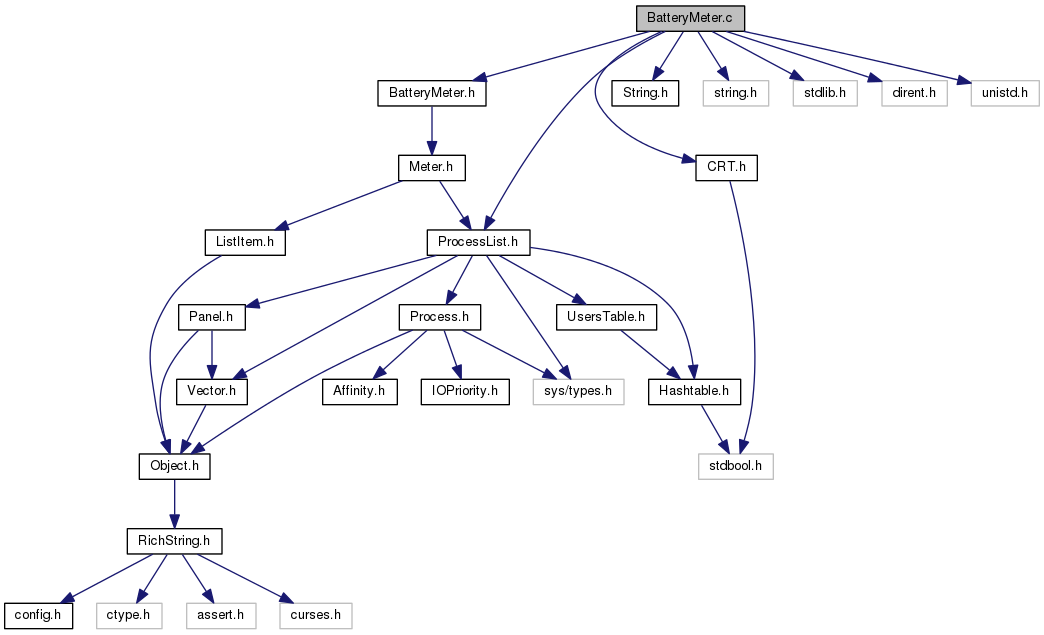
\includegraphics[scale=0.45]{res/battery_meter.png}
\caption{Граф включения для файла BatteryMeter.c}
\end{figure}

\newpage
%------------------------------------------------
\section{Мониторинг времени}

Монитор времени отвечает за отображение текущего времени пользователя. Отрывок файла ClockMeter.c представлен в листинге 4 а граф включения на рисунке 5.

Интерес представляет только одна функция. Она берёт локальное время (стр. 3) и преобразует его к привычному виду (часы:минуты:секунды), сохраняя это преобразование в буфере, который является аргументом функции.

\lstinputlisting[firstline=22,lastline=28,language=C++, caption={Clock Meter - мониторинг времени}]{../../top/ClockMeter.c}

\begin{figure}[h!]
\centering
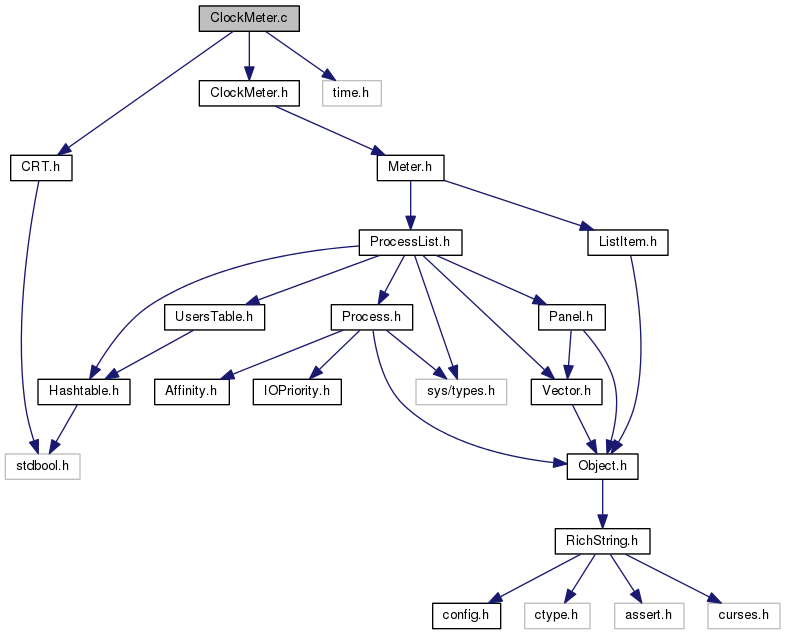
\includegraphics[scale=0.5]{res/clock_meter.png}
\caption{Граф включения для файла ClockMeter.c}
\end{figure}

\newpage
%------------------------------------------------
\section{Центральный процессор}

С оценкой потребления процессора всегда встает сложность разделения физических и логических ядер. В одном реальном процессоре может быть несколько ядер, каждое из которых может иметь дополнительный набор регистров, обеспечивающих hyper-threading.

Ранее мы рассматривали как происходит чтение информации об использовании процессора приложениями. Функция CPUMeter\_setValues из листинга 5 занимается подготовкой следующих полей:
\begin{itemize}
\item nicePeriod (стр. 11) - означает процент CPU, используемого пользовательскими процессами, на которые повлияло использование команд nice или renice, т.е. по существу их приоритет был изменен по сравнению с приоритетом по умолчанию, назначаемому планировщиком, на более высокий или низкий. При назначении какому-либо процессу команды nice, положительное число означает более низкий приоритет (1 = 1 шаг ниже нормального), а отрицательное число означает более высокий приоритет. 0 -- значение по умолчанию, что означает, что решение о приоритете принимает планировщик. Можно установить, какой планировщик используется системой.
\item userPeriod (стр. 12) - оказывает использование отдельного процессора (пользовательскими процессами, такими, как apache, mysql и т.д.) до максимального значения, составляющего 100\%. Таким образом, если в четырехъядерном процессоре 1 процесс использует 100\% CPU, это даст значение \%us, равное 25\%. Значение 12,5\% для 8-ядерного процессора означает, что занято одно ядро.
\item systemPeriod (стр 14) - означает использование CPU системой. Обычно это значение невысоко, высокие его значения могут свидетельствовать о проблеме с конфигами ядра, проблему со стороны драйвера, или целый ряд других вещей.
\item irqPeriod (стр 15) - означает прерывания на уровне железа; на плате электроны движутся по микросхемам предсказуемым образом. Например, когда сетевая карта получает пакет, перед передачей информации, содержащейся в пакете в процессор через ядро, она запросит прерывание в канале прерывания материнской платы. Процессор сообщает ядру, что у сетевой карты для него есть информация, а ядро имеет возможность решить, как поступить. Высокое значение времени, тратящегося на обработку прерываний на уровне железа встречается на виртуальной машине довольно редко, но по мере того, как гипервизоры предоставляют в распоряжение виртуальных машин все больше «железа», эта ситуация может измениться. Чрезвычайно высокая пропускная способность сети, использование USB, вычисления на графических процессорах, -- все это может привести к росту этого параметра на величину, превышающую несколько процентов.
\item softIrqPeriod (стр 16) - прерывание на уровне софта; начиная с ядра linux версии 2.4 реализована возможность запроса прерывания программным обеспечением (приложениями), а не элементом аппаратного обеспечения или устройством (драйвером), запрашивающим прерывание в канале прерывания материнской платы; запрос обслуживается ядром посредством его обработчика прерываний. Это означает, что приложение может запросить приоритетный статус, ядро может подтвердить получение команда, а программное обеспечение будет терпеливо ждать, пока прерывание не будет обслужено. Если мы применим утилиту tcpdump к гигабитному каналу с высоким трафиком, то значение может измениться примерно на 10\%, -- по мере заполнения выделенной памяти tcpdump, утилита посылает зарос на прерывание, чтобы переместить данные со стека на диск, экран и т.д. 
\item ioWaitPeriod (стр 17) - процент времени (циклов, секунд), в течение которого процессор простаивал, ожидая завершения операции ввода-вывода. Когда какой-либо процесс или программа запрашивает данные, он сначала проверяет кэш процессора (в нем имеется 2 или 3 кэша), затем проверяет память и, наконец, доходит до диска. Дойдя до диска, процессу или программе обычно приходится ждать, пока поток ввода-вывода передаст информацию в оперативную память, прежде чем иметь возможность снова на нем работать. Чем медленнее диск, тем выше будет значение IO Wait \% для каждого процесса. Это происходит также с процессами записи на диск, если системный буфер заполнен и его необходимо прочистить при помощи ядра – обычно это наблюдается на серверах баз данных с высокой нагрузкой. Если значение IO Wait стабильно превышает {100 / (кол-во CPU * кол-во процессов)}\%, это означает, что, возможно, имеется проблема хранения, с которой необходимо разобраться. Если вы наблюдаете высокую среднюю нагрузку, прежде всего, проверьте этот параметр. Если он высок, тогда узкое место в процессах, скапливающихся на диске, а не в чем-либо еще.
\item stealPeriod (стр 18) - в виртуализированной среде множество логических серверов могут работать под одним фактическим гипервизором. Каждой виртуальной машине(VM) присваивается 4-8 "виртуальных" CPU; хотя сами гипервизоры могут не иметь (кол-во VM * кол-во виртуальных CPU на одну VM). Причина этого заключается в том, что мы не перегружаем CPU использованием виртуальных машин, так что если дать одной-двум VM возможность изредка использовать 8 процессоров, это не будет негативно влиять на весь пул в целом. Однако если виртуальными процессорами VM используется количество CPU, превышающее количество физических (или логических, в случае с гиперпотоковыми процессорами Xeon), тогда значение iosteal будет расти.
\item guestPeriod (стр 19) - параметр похож на предыдущий, но со стороны виртуальной машины.
\end{itemize}

Функция CPUMeter\_display (стр. 33) занимается оформленным выводом информации, которую мы описали выше. Граф включения представлен на рисунке 6.

\lstinputlisting[firstline=45,lastline=126,language=C++, caption={CPU Meter - центральный процессор}]{../../top/CPUMeter.c}

\begin{figure}[h!]
\centering
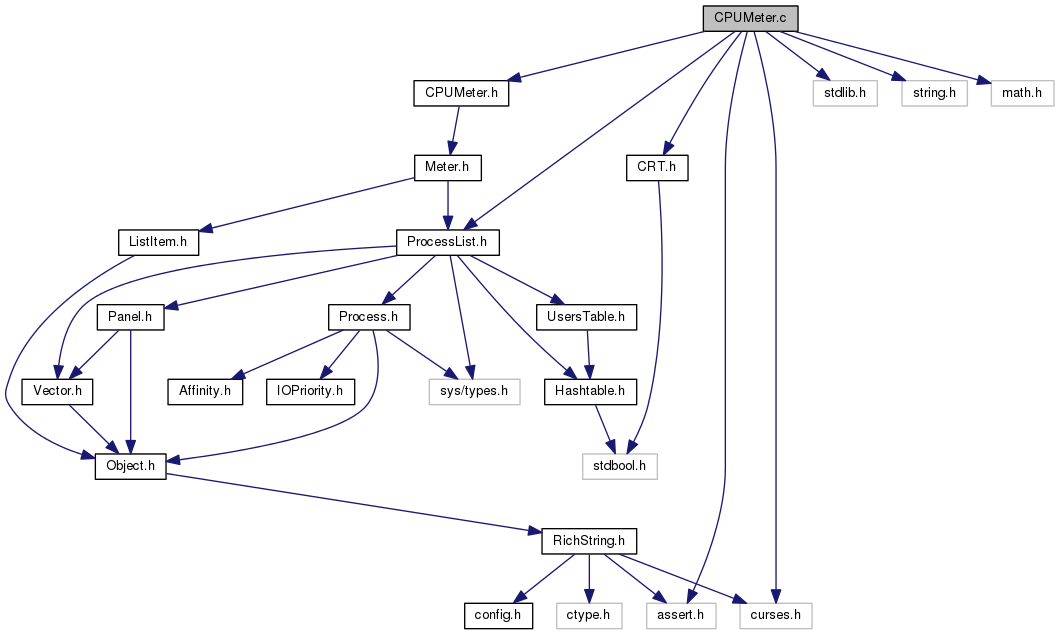
\includegraphics[scale=0.45]{res/cpu_meter.png}
\caption{Граф включения для файла CPUMeter.c}
\end{figure}

\newpage
%------------------------------------------------
\section{Имя устройства (хоста)}

Этот модуль является самым простым. Его работа сводится фактически к одной строке, которая записывает имя хоста в переданный буфер. Функция gethostname является стандартной (POSIX), и она определена в заголовочном файле unistd.h. Вызов этой функции обёрнут другой функцией HostnameMeter\_setValues, которая показана в листинге 5. Простота этой функции не отменяет её значимости, которая показана в графе включения на рисунке 7.

\lstinputlisting[firstline=22,lastline=25,language=C++, caption={Hostname Meter - имя устройства (хоста)}]{../../top/HostnameMeter.c}

\begin{figure}[h!]
\centering
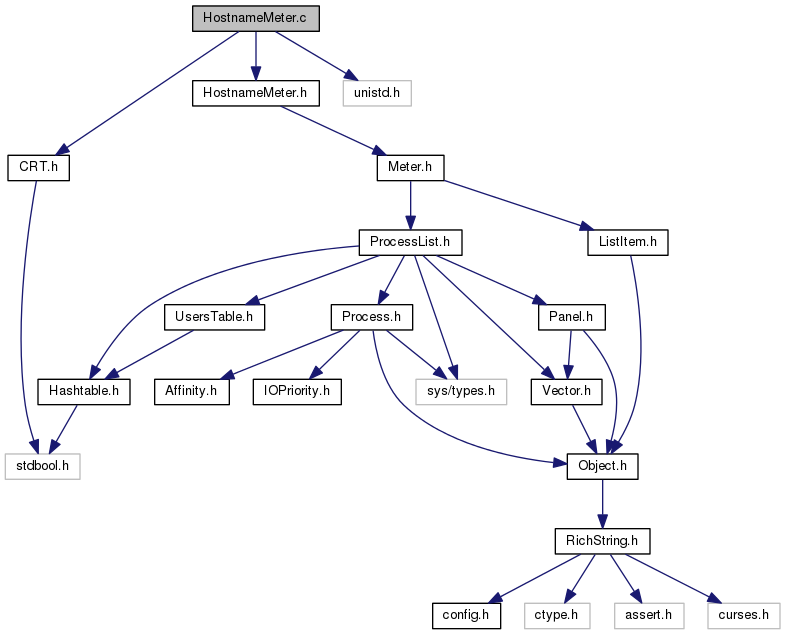
\includegraphics[scale=0.6]{res/hostname_meter.png}
\caption{Граф включения для файла HostnameMeter.c}
\end{figure}

\newpage
%------------------------------------------------
\section{Измерение средней загрузки}

Большую часть задачи, как и раньше, берёт на себя ядро. В файловой системе proc оно создаёт файл loadavg. Этот файл состоит из пяти групп:
\begin{itemize}
\item первое поле (число) — показывает использование процессора за последнюю минуту;
\item второе поле (число) — показывает использование процессора за последние пять минут;
\item третье поле (число) — показывает использование процессора за последние десять минут;
\item четвёртое поле (число/число) — состоит из двух значений, разделённых слешем, первая часть значения поля показывает количество выполняющихся в данный момент процессов/потоков (это значение не может быть больше количества присутствующих в системе CPU), вторая часть поля отображает количество процессов присутствующих в системе;
\item пятое поле (число) — хранит ID последнего запущенного в системе процесса (если для просмотра содержимого /proc/loadavg была использована команда cat, то будет значение PID именно программы cat).
\end{itemize}

В листинге 6 представлен отрывок файла LoadAverageMeter.c. Функция LoadAverageMeter\_scan (стр. 1) как раз обеспечивает открытие файла loadavg (стр. 4) и чтение пяти рассмотренных выше полей (стр. 6), при этом четвёртое поле читается как два различных числа.

Функция LoadAverageMeter\_setValues (стр. 14) обращается к LoadAverageMeter\_scan и сохраняет полученные значения по загрузке процессора за последнюю минуту, пять минут и десять минут в буфер (стр. 16), переданный в качестве аргумента.

Для отображения значений используется функция LoadAverageMeter\_display (стр 19). Она обеспечивает форматированный и цветной вывод для отображения загрузки процессора за последнюю минуту (стр. 22), пять минут (стр. 24) и десять минут (стр. 26).

Функции LoadMeter\_setValues (стр. 30) и LoadMeter\_display (стр 39) также обращаются к функции LoadAverageMeter\_scan, но они отображают только загрузку за последнюю минуту, для просмотра изменения загрузки в режиме (относительно) реального времени.

\newpage
\lstinputlisting[firstline=25,lastline=68,language=C++, caption={Load Average Meter - измерение средней загрузки}]{../../top/LoadAverageMeter.c}

\begin{figure}[h!]
\centering
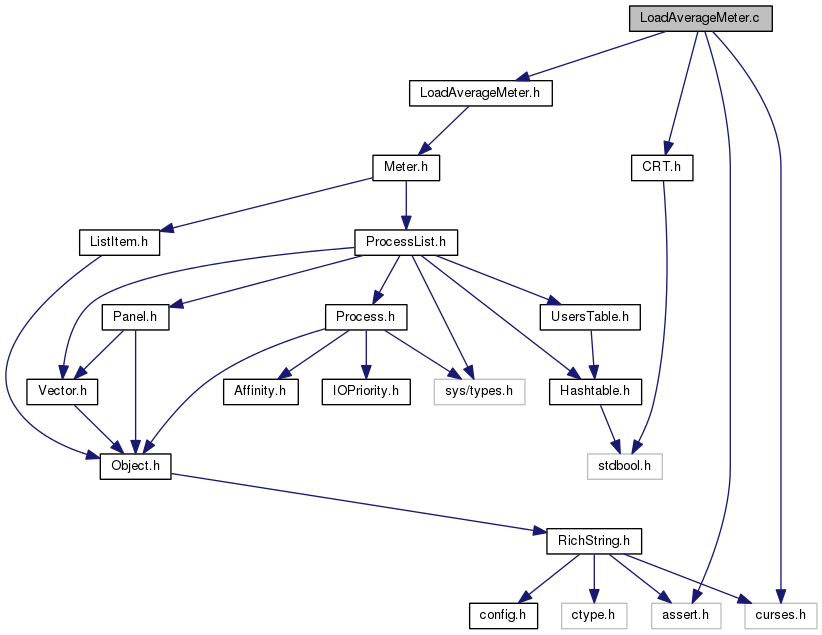
\includegraphics[scale=0.55]{res/load_average_meter.png}
\caption{Граф включения для файла LoadAverageMeter.c}
\end{figure}

\newpage
%------------------------------------------------
\section{Измерение уровня использования памяти}

Сбор различных характеристик системы уже был показан в листинге 2. В листинге 8 представлены две функции.

Функция MemoryMeter\_setValues (стр. 1) выводит в буфер следующую информацию:
\begin{itemize}
\item usedMem (стр. 2) - реально использующая в данный момент и зарезервированная системой память;
\item buffersMem (стр. 3) - буферы в памяти это страницы памяти, зарезервированные системой для выделения их процессам, когда они затребуют этого, так же известна как heap-memory;
\item cachedMem (стр. 4) - файлы, которые недавно были использованы системой/процессами и хранящиеся в памяти на случай если вскоре они снова потребуются.
\end{itemize}

Функция MemoryMeter\_display (стр. 13) занимается оформленным выводом собранной информации. Граф включения представлен на рисунке 9.

\lstinputlisting[firstline=28,lastline=60,language=C++, caption={Memory Meter - измерение уровня использования памяти}]{../../top/MemoryMeter.c}

\begin{figure}[h!]
\centering
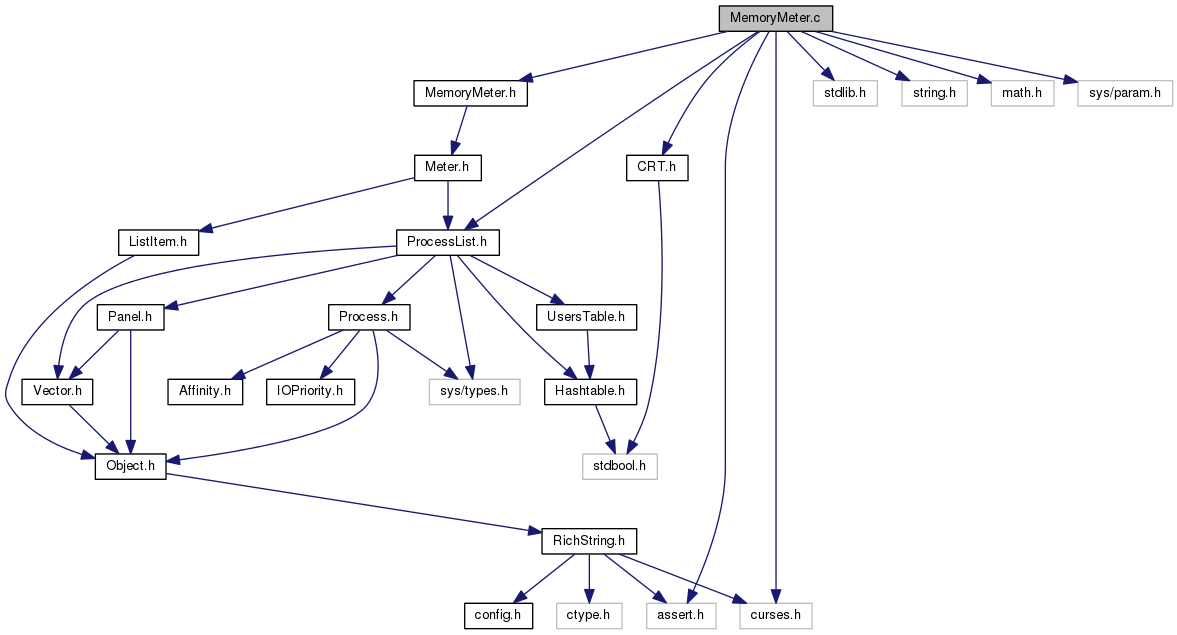
\includegraphics[scale=0.43]{res/memory_meter.png}
\caption{Граф включения для файла MemoryMeter.c}
\end{figure}

\newpage
%------------------------------------------------
\section{Измерение уровня использования области подкачки}

Если система приступает к запуску программу, которая требует больше оперативной памяти, чем доступно, то для решения этой задачи, используется технология swapping (”подкачка”). Суть этой технологии заключается в том, что некоторый объем данных (который не “помещается” в оперативную память) временно хранится на жестком диске, в то время как другая часть данных обрабатывается.

В Linux оперативная память делится на разделы, называемые страницами. Swapping (подкачка) – это процесс во время которого страницы памяти копируются на специально сконфигурированный для этого раздел диска, называемый swap space (раздел подкачки, может быть как и файлом, так и разделом жесткого диска), для освобождения ОЗУ. Совокупные размеры физической памяти и раздела подкачки – это объем имеющийся виртуальной памяти.

В листинге 2 мы рассматривали процедуру сбора системной информации, в листинге 9 нас интересуют три функции работы со свапом.

В функции SwapMeter\_humanNumber (стр. 2) размер раздела подкачки приводится к виду, легко воспринимаемому человеком. Если объём превышает 10 гигабайт, то число отображается как соответствующее количество гигабайт (стр 4). Если число превышает 10 мегабайт, то оно отображается как соответствующее количество мегабайт (стр 6). Если ни одно из предыдущих правил не сработало, то объём отображается в килобайтах (стр. 8).

Функция SwapMeter\_setValues (стр. 11) выводит информацию о подкачке в буфер, переданный в качестве параметра. Для этого используется общий объём свапа (стр. 13) и занятый объём (стр. 12).

Функция SwapMeter\_display (стр 18) обеспечивает форматированный вывод всей собранной информации. Граф включения представлен на рисунке 10.

\lstinputlisting[firstline=32,lastline=60,language=C++, caption={Swap Meter - измерение уровня использования области подкачки}]{../../top/SwapMeter.c}

\begin{figure}[h!]
\centering
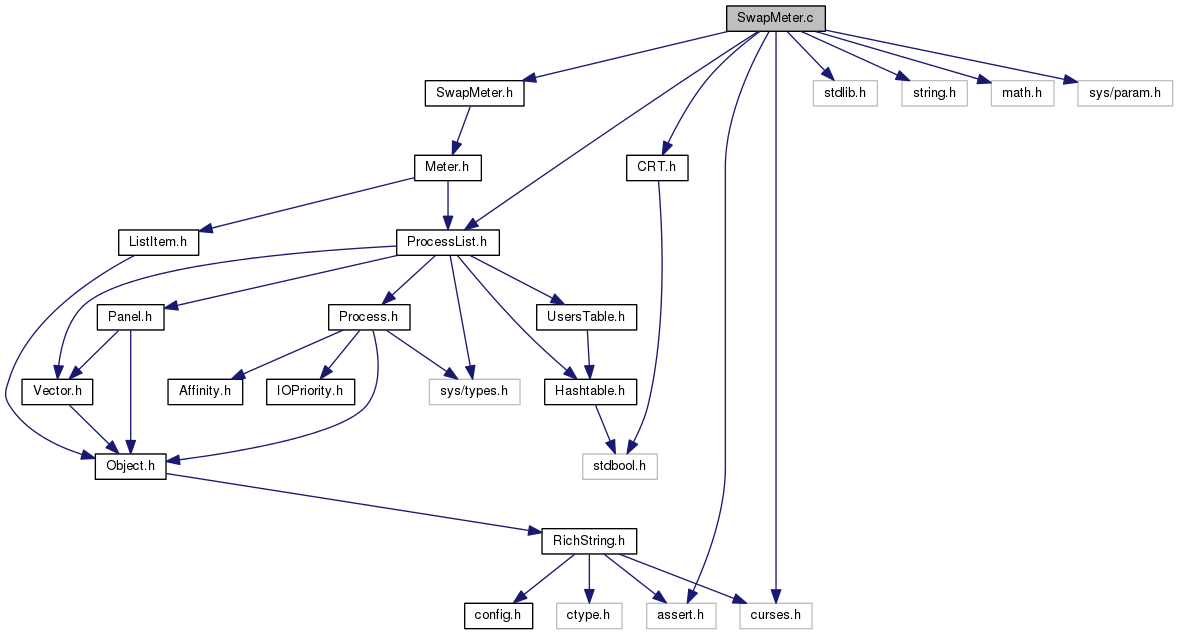
\includegraphics[scale=0.43]{res/swap_meter.png}
\caption{Граф включения для файла SwapMeter.c}
\end{figure}

\newpage
%------------------------------------------------
\section{Мониторинг процессов}

Как мы уже говорили, все процессы представлены своей директорией в файловой системе proc. вывод этой информации можно изучить в листинге 10.

Функция TasksMeter\_setValues (стр. 1) занимается в выводом в буфер (стр. 5) информации о процессах. Этой информацией является общее количество процессов (стр. 3) и количество запущенных в данный момент процессов (стр. 4). Как мы говорили выше, количество запущенных процессов не может превышать количество процессоров.

Функция TasksMeter\_display (стр. 8) обеспечивает форматированный вывод информации о процессах. При этом стоит обратить внимание, что она выводит не только процессы пользователя (стр. 22) но и процессы ядра (стр. 28), которые могут заниматься, к примеру, управлением кэшами.

Граф включений представлен на рисунке 11.

\lstinputlisting[firstline=21,lastline=56,language=C++, caption={Tasks Meter - мониторинг процессов}]{../../top/TasksMeter.c}

\begin{figure}[h!]
\centering
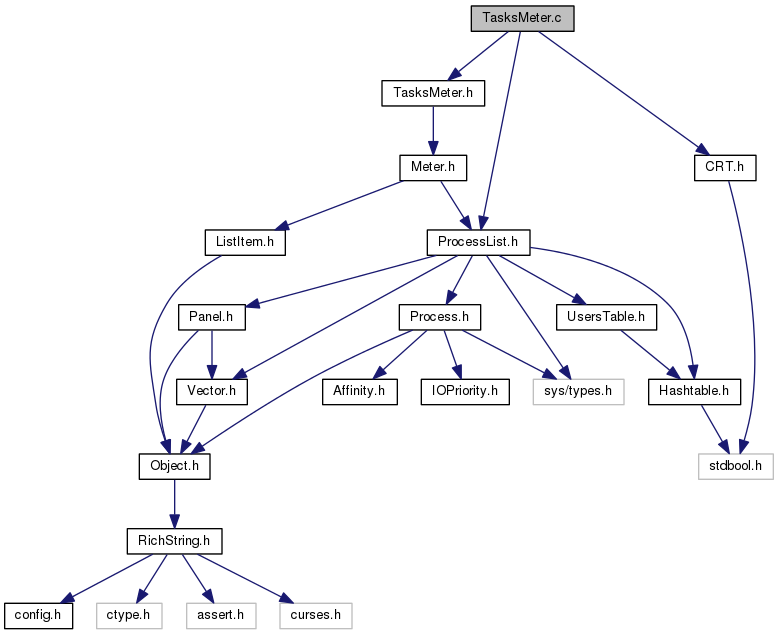
\includegraphics[scale=0.6]{res/tasks_meter.png}
\caption{Граф включения для файла TasksMeter.c}
\end{figure}

\newpage
%------------------------------------------------
\section{Измерение времени работы системы}

Время работы системы также хранится в файловой системе proc в файле uptime. В листинге 11 представлена функция UptimeMeter\_setValues (стр. 1), которая открывает этот файл (стр. 3) и считывает оттуда значение (стр. 5). Стоит отметить, что на самом деле в этом файле хранится два числа.

\begin{itemize}
\item первое показывает количество секунд, прошедших с момента включения компьютера (это значение используется в дальнейшем)
\item второе показывает количество времени (тоже в секундах), которое система провела в бездействии (в т.ч. ожидая завершения операций ввода-вывода); на многоядерных системах это число складывается из времени бездействия каждого ядра, так что второе число по значению может обогнать первое.
\end{itemize}

Число секунд с момента включения приводится к виду, удобному для человеческого восприятия - в буфер выводится (стр. 27) количество дней, часов, минут и секунд работы.

\lstinputlisting[firstline=24,lastline=51,language=C++, caption={Uptime Meter - измерение времени работы системы}]{../../top/UptimeMeter.c}

\begin{figure}[h!]
\centering
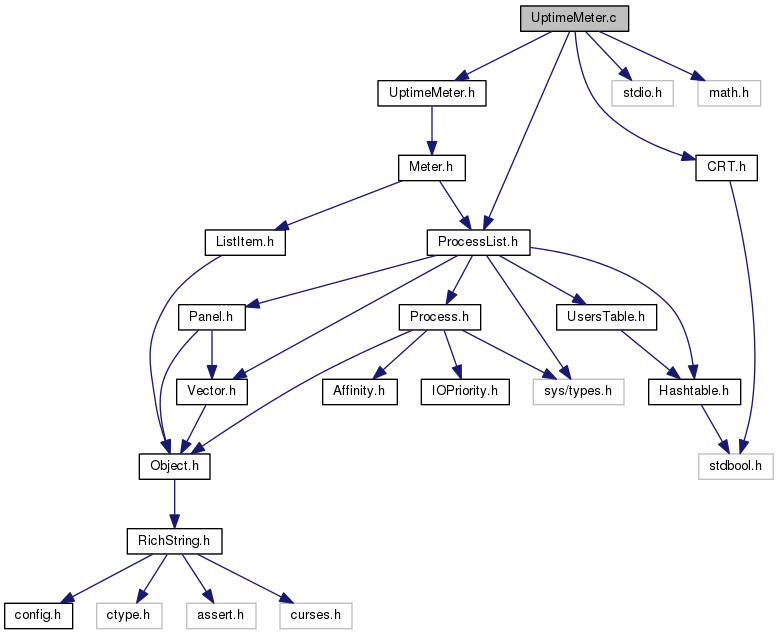
\includegraphics[scale=0.6]{res/uptime_meter.png}
\caption{Граф включения для файла UptimeMeter.c}
\end{figure}

\newpage
%------------------------------------------------
\section*{Заключение}
\addcontentsline{toc}{section}{Заключение}

В данной работе нами была изучена программа htop, являющееся расширенной версией стандартной утилиты top. Мы выпустили из рассмотрения особенности, связанные с графическим выводом (на базе библиотеки ncurces), сосредоточившись на основных функциональных возможностях.

Изучив исходный код, мы убедились, что никакие специальные системные вызовы утилита не использует, только самые широко распространённы, вроде чтения из файла и вывод на экран (но они используются так часто, что их систематизация для данного отчёта оказалась крайне затруднительной).

Основным выводом является тот факт, что в отличии от Windows, Linux предоставляет удобный механизм сбора системной информации через файловую систему proc.

\newpage
%------------------------------------------------
\section*{Список литературы}
\addcontentsline{toc}{section}{Список литературы}

\begin{enumerate}
\item Яремчук С. А.  Linux Mint на 100 \%. — СПб.: Питер, 2011. — 240 е.: ил. — (Серия «На 100 \%»). ISBN: 978-5-49807-803-8.
\item HowTo: Troubleshoot with linux 'top' command. David Van Rood (dowdandassociates.com). 
\end{enumerate}

\end{document}
